\section{Geometrische und thermische Grundlagen der Erwärmung mit Laser}

Zur Bestimmung der bei der Lasererwärmung eingetragenen Wärme ist die Betrachtung von zwei unterschiedlichen Teilaspekten notwendig: Zum Einen der Einfluss der Bewegungsgeschwindigkeit des Laserflecks, zum Anderen derjenige der Eigenschaften des verwendeten Werkstoffes.

\subsection{Geschwindigkeit des Laserbrennflecks}

Zur Bestimmung der Geschwindigkeit des Laserflecks wird das System in dreidimensionalen Koordinaten betrachtet. In diesen Koordinaten stellt sich die Bewegungsgeschwindigkeit $\vv{v_t}$ des Werkzeugs dar als:
\begin{equation}
 \vv{v_t} = \left(\begin{array}{c}v_{t,x}\\v_{t,y}\\0\end{array}\right)
 \label{eqn:toolvel3d}
\end{equation}

Weiterhin gilt für die Winkelgeschwindigkeit $\vv{\dot{\varphi}}$ der Bewegung des Laserflecks:
\begin{equation}
 \vv{\dot{\varphi}} = \left(\begin{array}{c}0\\0\\\dot{\varphi}\end{array}\right)
 \label{eqn:laserrotvel3d}
\end{equation}
 
Zudem ergibt sich aus der Geometrie des Aufbaus %(Abbildung \ref{img:geovel})
für den Radialvektor $\vv{r}$ mit der Entfernung $d_l$ des Laserflecks von der Rotationsachse:
\begin{equation}
\vv{r} = d_l\left(\begin{array}{c}-\sin\varphi\\\cos\varphi\\0\end{array}\right)
\label{eqn:radvec3d}
\end{equation}

% \begin{figure}[htbp]
%  \centering
%  \begin{pspicture}(8,5)
%   \psline{->}(4,1)(8,1)
%   \rput(8,0.6){x}
%   \psline{->}(4,1)(4,5)
%   \rput(3.6,5){y}
%   {
%    \SpecialCoor
%    \rput(4,1)
%    {
%     \psline(3.5;90)(0,0)(3.5;120)
%     \psarc{->}(0,0){3}{90}{120}
%     \rput[br](3.1;105){$\varphi$}
%    }
%   }
%  \end{pspicture}
%  \caption{Geometrie der Anordnung des Laserflecks}
%  \label{img:geovel}
% \end{figure}

Für den Geschwindigkeitsvektor $\vv{v_l}$ des Laserflecks gilt nun:
\begin{equation}
 \vv{v_l} = \vv{v_t} + \vv{\dot{\varphi}} \times \vv{r}
 \label{eqn:dotvelcomp}
\end{equation}

Einsetzen von Gleichungen \ref{eqn:toolvel3d}, \ref{eqn:laserrotvel3d} und \ref{eqn:radvec3d} in Gleichung \ref{eqn:dotvelcomp} und Umformen ergibt:
\begin{equation}
 \vv{v_l} = \left(\begin{array}{c}v_{t,x}\\v_{t,y}\\0\end{array}\right) - d_l\; \dot{\varphi} \left(\begin{array}{c}\cos\varphi\\\sin\varphi\\0\end{array}\right)
 \label{eqn:dotvelfin3d}
\end{equation}

Da das Problem im Prinzip zweidimensional ist und in Gleichung \ref{eqn:dotvelfin3d} die dritte Komponente immer null ist, liegt es nahe, die Gleichung in zwei Dimensionen darzustellen:
\begin{equation}
 \vv{v_l} = \left(\begin{array}{c}v_{t,x}\\v_{t,y}\end{array}\right) - d_l\; \dot{\varphi} \left(\begin{array}{c}\cos\varphi\\\sin\varphi\end{array}\right)
 \label{eqn:dotvelfin2d}
\end{equation}

Interessant ist jedoch nur der Betrag der Geschwindigkeit des Laserflecks, welcher sich wie folgt bestimmt:
\begin{equation}
 v_l = \left|\vv{v_l}\right| = \sqrt{\left(v_{t,x} - d_l\dot\varphi\cos\varphi\right)^2 + \left(v_{t,y} - d_l\dot\varphi\sin\varphi\right)^2}
 \label{eqn:dotvelabs}
\end{equation}

\label{sec:geotheory}

\subsection{Durch Laserstrahlung eingetragene Wärme}

Die Strahlungsenergie des Lasers wird im Blech in innere Energie in Form von Wärme umgewandelt. Laut \cite{atkins} gilt für die infinitesimale Temperaturänderung $dT$ durch die Änderung der inneren Energie $dU$ bei der spezifischen Wärmekapazität $C_{V,s}$ und konstantem Volumen:
\begin{equation}
  dT = \frac{dU}{mC_{V,s}}
  \label{eqn:specificheat}
\end{equation}

wobei $m$ die Masse des erwärmten Stoffes darstellt. Auf einem Teil eines Bleches der Dicke $d_s$, welches die Länge $l_e$ und die Breite $b_e$ besitzt (s. Abbildung \ref{img:element}), bestimmt sich die Masse über die Dichte $\rho$ zu:

\begin{equation}
 m = \rho V = \rho d_s l_e b_e
 \label{eqn:massgeometry}
\end{equation}

\begin{figure}[!btp]
 \centering
 \includegraphics[width=0.8\textwidth]{images/element}
 \caption{Skizze eines Volumenelements zur Bestimmung der Wärmekapazität}
 \label{img:element}
\end{figure}

Mit dieser Beziehung und Gleichung \ref{eqn:specificheat} ergibt sich für die Änderung der Temperatur:
\begin{equation}
  dT = \frac{dU}{\rho d_s l_e b_eC_{V,s}}
  \label{eqn:tempgeometry}
\end{equation}

Weiterhin ist die Leistung $P$ definiert als die Änderung der Energie mit der Zeit, also gilt:
\begin{equation}
  P = \frac{dU}{dt}\;\;\Leftrightarrow\;\; dU = Pdt
  \label{eqn:definitionpower}
\end{equation}

Laut \cite{laserheating} gilt für die absorbierte Leistung $P_a$:
\begin{equation}
  P_a = \alpha P_g
  \label{eqn:absorptivity}
\end{equation}

mit dem Absorptionsgrad $\alpha$ und der gesamten eingestrahlten Leistung $P_g$. Diese wiederum lässt sich mit $b_e'$, der Breite des vom Laserflecks getroffenen Teil des betrachteten Blechteils, sowie der Breite des gesamten Laserflecks $b_l$ und der Laserleistung $P_l$ abschätzen zu:
\begin{equation}
  P_g = \frac{b_e'}{b_l}P_l
  \label{eqn:powerfrac}
\end{equation}

Hierbei wird davon ausgegangen, dass die Laserleistung über die gesamte Breite des Laserflecks gleichverteilt ist. Einsetzen von Gleichung \ref{eqn:powerfrac} in Gleichung \ref{eqn:absorptivity} und dieser in \ref{eqn:definitionpower} ergibt:
\begin{equation}
  dU = \frac{b_e'}{b_l}\alpha P_l dt
  \label{eqn:energyofpower}
\end{equation} 

Dies wiederum ergibt mit Gleichung \ref{eqn:tempgeometry} einen Zusammenhang zwischen der Temperaturänderung und der Laserleistung:
\begin{equation}
  dT = \frac{1}{\rho d_s l_e b_eC_{V,s}} \frac{b_e'}{b_l}\alpha P_l dt = C \frac{b_e'}{b_l}\alpha P_l dt
  \label{eqn:dTofdt}
\end{equation}

Hierbei ist $C = \frac{1}{\rho d_s l_e b_eC_{V,s}}$ mit der Zeit konstant. Integrieren beider Seiten von $t'=0$ bis $t'=t$ ergibt:
\begin{equation}
  \Delta T = \int_{T(0)}^{T(t)} dT = \int_{0}^{t} C \frac{b_e'}{b_l}\alpha P_l dt' = C \frac{b_e'}{b_l} P_l \int_{0}^{t} \alpha dt'
  \label{eqn:integrationtemp}
\end{equation}

Dies ist zulässig, da laut \cite{laserheating} nur der Absorptionsgrad sich zwischen Raumtemperatur und Schmelztemperatur eines Metalls maßgeblich ändert. Dieser lässt sich mit der folgender Näherung beschreiben:

\begin{equation}
\alpha(T) = \alpha_0 + \alpha_1 T
\end{equation}

Dies würde jedoch eine Integration der rechten Seite von Gleichung \ref{eqn:integrationtemp} sehr kompliziert machen. Daher wird ein vereinfachter Absorptionsgrad $\alpha'$ eingeführt, der das Gesamtergebnis der Integration nicht beeinflusst, diese jedoch deutlich vereinfacht. Dazu lässt sich Gleichung \ref{eqn:dTofdt} umformen zu:

\begin{equation}
 \frac{\rho d_sl_eb_eC_{V,s}b_l}{b_e'}\frac{dT}{\alpha(T)} = c \frac{dT}{\alpha_0 + \alpha_1 T} = P_l dt
 \label{eqn:alphaintpreconst}
\end{equation}

wobei $c = \frac{\rho d_sl_eb_eC_{V,s}b_l}{b_e'P_l}$ als temperaturunabhängig gesehen werden kann. Integration ergibt:
\begin{equation}
  \int_{T_R}^{T_Z}c\frac{dT}{\alpha_0 + T \alpha_1} = c\frac{\ln\left(\alpha_0 T_Z + \alpha_1\right)-\ln\left(\alpha_0 T_R + \alpha_1\right)}{\alpha_1} = \Delta U = \int_0^t P_l dt'
\end{equation}

Wird nun $\alpha'$ eingeführt als 

\begin{equation}
\alpha' = \frac{\alpha_1 \Delta' T}{\ln\left(\alpha_0 T_Z + \alpha_1\right)-\ln\left(\alpha_0 T_R + \alpha_1\right)}
\label{eqn:alphas}
\end{equation}

mit $\Delta'T = T_Z-T_R$ der Differenz zwischen Zieltemperatur und Raumtemperatur, so ergibt sich, dass ein Ersetzen von $\alpha$ durch $\alpha'$ bei der Betrachtung der gesamten Temperaturdifferenz keinen Fehler einführt.

\begin{eqnarray}
  \int_{T_R}^{T_Z}c\frac{dT}{\alpha'} &=& c\int_{T_R}^{T_Z}\frac{\ln\left(\alpha_0 T_Z + \alpha_1\right)-\ln\left(\alpha_0 T_R + \alpha_1\right)}{\alpha_1 \Delta' T} dT\\\nonumber
   &= &c\frac{\ln\left(\alpha_0 T_Z + \alpha_1\right)-\ln\left(\alpha_0 T_R + \alpha_1\right)}{\alpha_1}\\
   &= &\int_{T_R}^{T_Z}c\frac{dT}{\alpha}
\end{eqnarray}

Somit kann durch diese vereinfachte Betrachtung die Entwicklung der Temperatur zwischen Raumtemperatur und Zieltemperatur nicht vorhergesagt werden. Dies führt in diesem Fall jedoch nicht zu Problemen, da einzig die zuzuführende Wärmemenge ausschlaggebend ist, die zur Zieltemperatur führt. Diese allerdings wird korrekt bestimmt. Für die Temperaturdifferenz ergibt sich:
\begin{equation}
  \Delta T = \frac{1}{\rho d_s l_e b_e C_{V,s}} \frac{b_e'}{b_l} P_l \alpha' \int_{0}^{t}  dt' = \frac{1}{\rho d_s l_e b_e C_{V,s}} \frac{b_e'}{b_l} P_l \alpha' t
  \label{eqn:integrated}
\end{equation}

Hier beschreibt $t$ die Zeit, in welcher der Laserstrahl das betrachtete Element über\-streicht. Diese lässt sich berechnen nach:
\begin{equation}
  t = \frac{l_e}{v_l}
  \label{eqn:elementtime}
\end{equation}

Somit wird Gleichung \ref{eqn:integrated} zu:
\begin{equation}
  \Delta T = \frac{\alpha'}{\rho d_s b_e C_{V,s}} \frac{b_e'}{b_l} \frac{P_l}{v_l}
  \label{eqn:prefinal}
\end{equation}

Da im Allgemeinen gilt $b_e << b_l$, ist davon auszugehen, dass der Effekt, der dadurch entsteht, dass jeweils zwei Elemente nur zum Teil vom Laserfleck überstrichen werden, gering ist, sich also $b_e' \approx b_e$ annehmen lässt. Somit ergibt sich aus Gl \ref{eqn:prefinal}
\begin{equation}
  \Delta T = \frac{\alpha'}{\rho d_s C_{V,s}b_l} \frac{P_l}{v_l} = c_P \frac{P_l}{v_l}\;\;\mbox{mit}\; c_P = \frac{\alpha'}{\rho d_s C_{V,s}b_l}
  \label{eqn:final} 
\end{equation}

wobei $c_P$ eine Konstante ist, die sich für den gesamten Prozess nicht ändert. Somit hängt die Temperaturdifferenz nur noch von der Laserleistung und der Geschwindigkeit des Laserbrennflecks ab.
\label{sec:heattheory}
